\section{Msza Święta}

\subsection{Przed Mszą Św.}

Należy przyjść odpowiednio wcześniej. Osoby funkcyjne proszone są o zapoznanie
się ze swoimi czynnościami. Zakrystianie muszą wcześniej upewnić się, że
wszystkie przedmioty są na odpowiednich miejscach i w odpowiednich momentach
mszy zadbać o wypisane przedmioty.

\subsection{Wejście}

\begin{itemize}
      \item Procesja wejścia ustawia się następująco:
            \begin{center}
                  \uparrow \smallskip\\
                  \tt1~~~\cc3 \smallskip\\
                  \aa2~\ding{63}~\aa1 \smallskip\\
                  M~~~M \smallskip\\
                  M~~~M \smallskip\\
                  M~~~M \smallskip\\
                  \cc1 \smallskip\\
                  \ii
            \end{center}
      \item Po przyjściu do ołtarza \aa\aa~ nie klękają, ale kłaniają się, bo jest
            między nimi \ding{63}.
      \item Gdy tabernakulum jest puste reszta ministrantów ilekroć przechodzi
            przez środek przyklęka, tylko celebrans wykonuje głęboki skłon.
      \item Modlitwy u stopni ołtarza bez psalmu \textit{Iudica me}
\end{itemize}

\subsection{\textit{Gloria} i \textit{Credo}}

\begin{itemize}
      \item Na hymn \textit{Gloria} \zz~ oraz \tt1 dzwonią sygnaturkami do czasu
            odmówienia go przez \ii.
      \item Po odśpiewaniu \textit{Gloria} miejsce dzwonków zastępują kołatki.
      \item Opuszcza się \textit{Credo}
\end{itemize}

\subsection{Lucenarium}

\begin{itemize}
      \item Do lucenarium wyznacza się 6 ministrantów, którzy po okadzeniu ludu
            ustawiają się parami w kierunku ołtarza.
      \item Na wyraźny znak \cc2 przyklękają i udają się do bocznej nawy po
            pochodnie.
      \item Na śpiew \textit{Sanctus} bardzo powoli zmierzają do prezbiterium. Na
            wysokości sedilli rozchodzą się na boki.
      \item Na znak \cc2 przyklękają a następnie klękają na oba kolana.
      \item Nie wstają na słowa \textit{Per omnia secula seculorum}, ale czekają na
            obrzędy komunii.
      \item W czasie formowania się procesji komunijnej wstają i obracają się
            twarzami do siebie tak, aby stworzyć przejście. Osoba w środku staje
            się osią obrotu dla każdej trójki.
      \item W takim stanie pozostają aż do procesji do ciemnicy. Pochodnie
            trzymają w prawej ręce.
      \item W czasie całego kanonu nie reagują na to, co dzieje się na ołtarzu,
            tj. nie skłaniają głowy na Przeistoczenie.
\end{itemize}

\subsection{\textit{Kanon} i Komunia Św.}

\begin{itemize}
      \item \cc3 w czasie śpiewu \textit{Sanctus} rozdaje świece ministrantom a
            pod koniec kanonu daje znak, aby je zgasić.
      \item \cc3 idzie z ogniem do wiernych: na początku na śpiew Sanctus a potem
            po przyjęciu Komunii.
      \item Na śpiew \textit{Agnus Dei} odpowiada się trzykrotnie
            \textit{Miserere nobis}.
      \item Podczas śpiewu \textit{Agnus Dei} \aa1 bierze z kredencji obrus
            komunijny, razem z \aa2 klękają pośrodku, wchodząc na najwyższy
            stopień ołtarza i klęcząc przodem do siebie trzymają rozłożony obrus.
      \item Ministranci pozostający w chórze tworzą dwójkami w sposób naturalny
            „kolejkę” do Komunii św.
            \begin{figure}[h!]
                  \centering
                  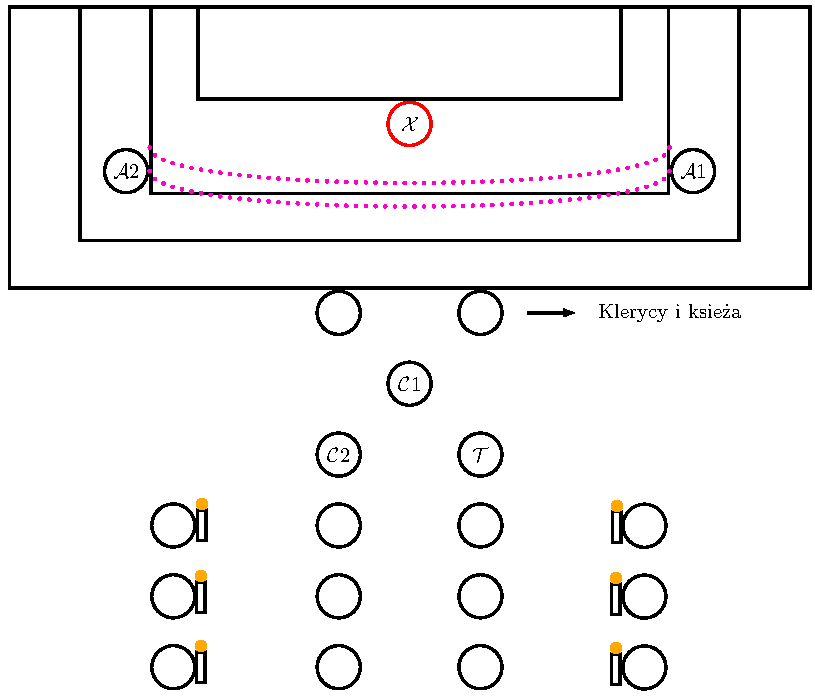
\includegraphics[width=0.5\linewidth]{Figures/Czwartek/Komunia1.pdf}
                  \caption{Przyjmowanie Komunii Św. -- część 1}
            \end{figure}
      \item Przed nimi do kolejki wchodzą księża, klerycy i ceremoniarze, za nimi
            reszta ministrantów z chóru.
      \item \cc1 podaje patenę pierwszemu duchownemu przyjmującemu Komunię św.,
            albo, jeśli nie ma duchownych trzyma ją sam. Po przyjęciu Komunii Św.
            zajmuje miejsce przy \ii, gdzie asystuje z pateną.
      \item \cc2 po przyjęciu Komunii św. zajmuje miejsce przy celebransie ze
            świeczką sanctusową.
      \item \aa\aa~ trzymający obrus przyjmują Komunię św. razem po \cc.
            \begin{figure}[h!]
                  \centering
                  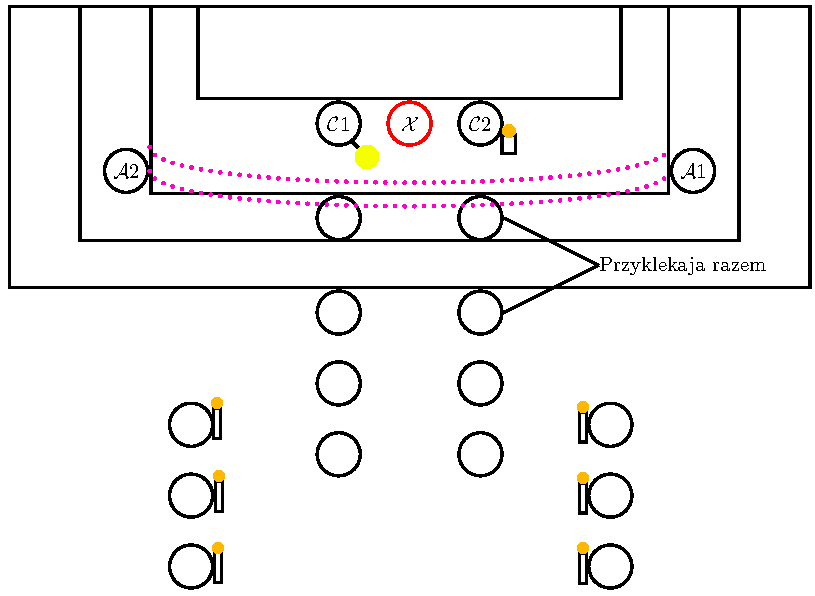
\includegraphics[width=0.5\linewidth]{Figures/Czwartek/Komunia2.pdf}
                  \caption{Przyjmowanie Komunii Św. -- część 2}
            \end{figure}
      \item Każda dwójka przystępująca do Komunii św. przyklęka jednocześnie z
            poprzedzającą parą, wchodzi na stopnie i klęka na dwa kolana. Po
            przyjęciu komunii znów przyklęka jednocześnie z parą stojącą za nimi.
            Ze stopni ołtarza schodzimy w lewo po stopniu diakońskim – do chóru.
      \item Po przyjęciu komunii zapala się znów świece, które trzymają aż do
            procesji do ciemnicy.
      \item Po komunii cały chór klęczy do słów \textit{Dominus vobiscum} z
            zapalonymi już świecami.
      \item \cc3 i \cc4 kierują porządkiem przyjmowania Komunii przez wiernych
            dbając o sprawne przystępowanie i odchodzenie
            \begin{figure}[h!]
                  \centering
                  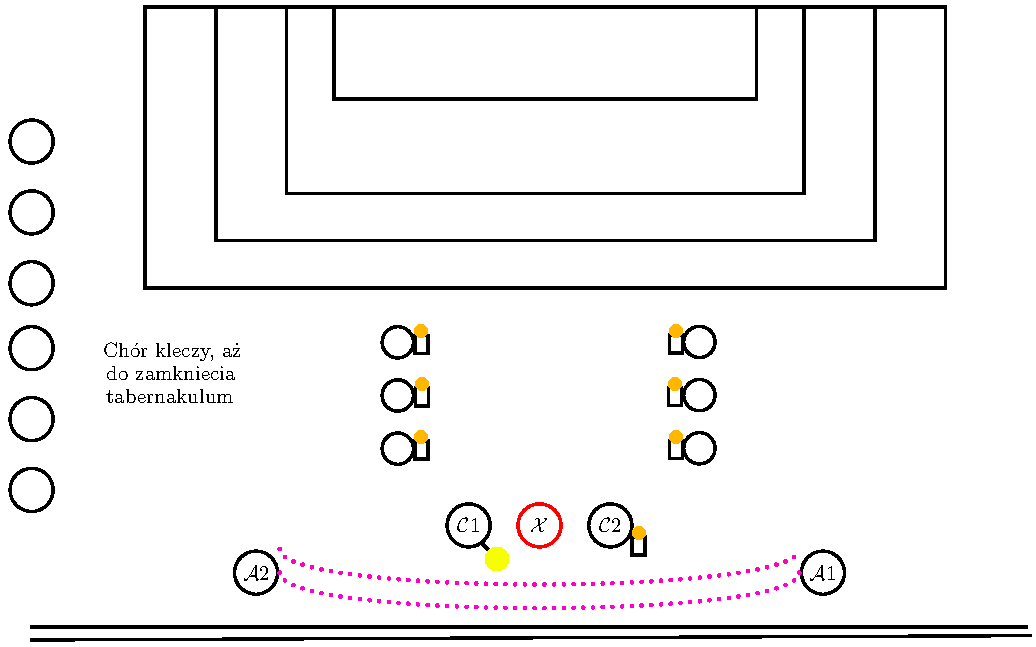
\includegraphics[width=0.5\linewidth]{Figures/Czwartek/Komunia3.pdf}
                  \caption{Przyjmowanie Komunii Św. -- część 3}
            \end{figure}
      \item Do ołtarza \aa\aa~ podchodzą bokiem, przyklękając raz na dole. Do
            przeniesienia mszału i welonu nie idą na skos, ale również bokiem. W
            czasie zabierania welonu i przenoszenia mszału \aa2 zabiera ze sobą
            białe rękawiczki do zniesienia kielicha.
\end{itemize}

\subsection{Zakończenie Mszy}

\begin{itemize}
      \item  Msza święta kończy się słowami \textit{Benedicamus Domino}, następnie
            \ii~ odmawia \textit{Placeat} i całuje ołtarz.
      \item Opuszcza się błogosławieństwo oraz ostatnią ewangelię.
\end{itemize}

